 

\documentclass{report}
%%%%%%%%%%%%%%%%%%%%%%%%%%%%%%%%%%%%%%%%%%%%%%%%%%%%%%%%%%%%%%%%%%%%%%%%%%%%%%%%%%%%%%%%%%%%%%%%%%%%%%%%%%%%%%%%%%%%%%%%%%%%



\usepackage{epigraph}
\usepackage[toc,page]{appendix}

\usepackage{graphicx} 

\newcommand{\ns}{\noindent }

\newcommand{\sh}[1]{\indent\indent\texttt{\footnotesize\$ #1}}
\newcommand{\shni}[1]{\texttt{\footnotesize\$ #1}}


 \textwidth = 400pt
 \textheight = 570pt
 \oddsidemargin =0 pt

\usepackage[colorlinks=true]{hyperref}



\begin{document}


\begin{titlepage}
    \centering
    \vfill
    {\bfseries\Large
        Toxic Comment Classification challenge\\
         Udacity Capstone - Machine Learning Engineering\\
        \vskip1cm
        R. Angeles\\
    }    
    \vfill
    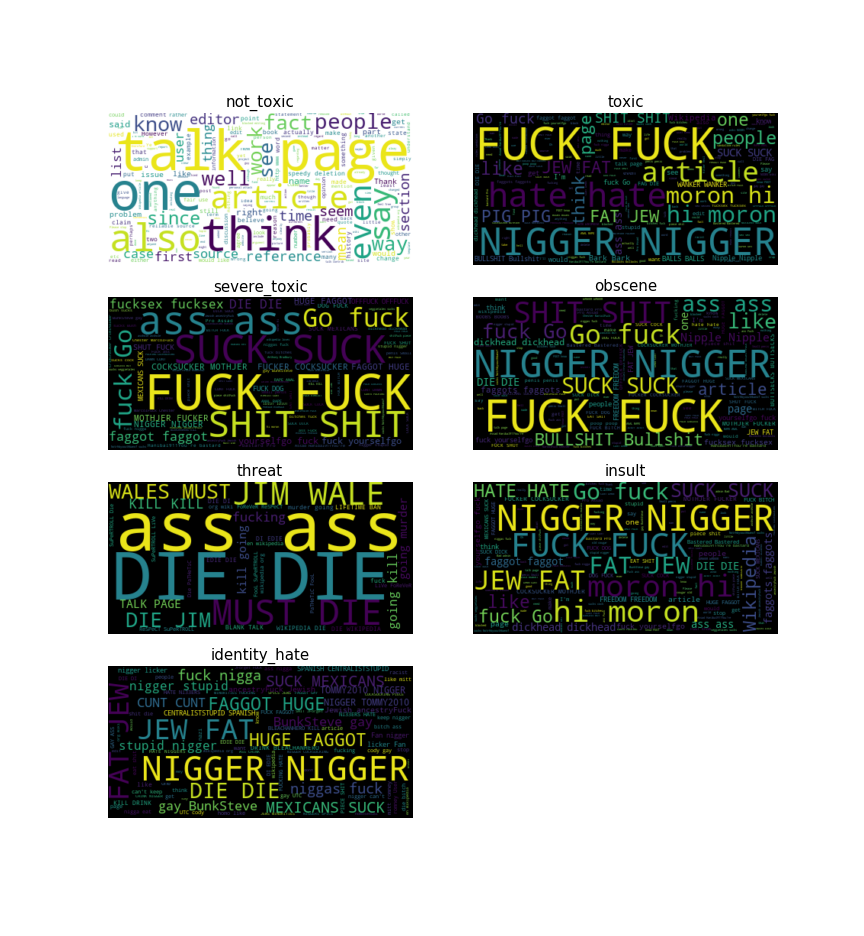
\includegraphics[width=15cm]{../local/plots_tables/clouds.png} % also works with logo.pdf
    \vfill
    \vfill
\end{titlepage}




\chapter{Definition}

\section{Overview}

In this project we work on the Kaggle toxic comment classification challenge that aims improving 
online conversation. In a nutshell, the challenge consist in build an ML model to classify 
Wikipedia, talk edits page, comments as being toxic, severe toxic, obscene, treat or identity hate.


\section{Problem Statement}

Our aim is to explore the performance of three well models for the analysis of
this data set: CNN, GRU and LSTM on top of the GLOVE pretrained word embedding. 
We not only aimed for a model that performs well but to deploy it  
on Sagemaker.

\section{Metrics, goals and reasults}

The benchmark analysis for comparison is the most voted
kernel of the competition: a Naive Bayes - Support Vector Machine model, it reaches 0.9772 auc roc,
while the current leader team reaches 0.98856. We manage to top such benchmark, but the main 
results of the work consist in exploring the performance three popular model for NLP:  CNN, LSTM and GRU.
When combined with a given preprocessing, and using the Glove pretrained word embedding our model tops 
our benchmark model under 10 mins, on a laptop.

In addition, we deploy the CNN model to an interactive website via SageMaker and on the road 
we create portable utilities to use the benefits Torchtext on Sagemaker pytorch containers. 
After presenting our analysis we discuss performance and future directions. 


\chapter{Analysis}


\section{Data Exploration}

 Jigsaw/Google/Kabble provide a training dataset  of 160K comments, with binary labels
 corresponding to the following classes:
 \emph{Toxic, Severe toxic, Obscene, Threat, Insult or  identity hate}.
 Additionally, a test dataset  with over 153K unlabelled  test comments is provided to make 
 a submission to the competition. The dataset is available at \cite{Kaggle}. This should be placed under a data
 directory to reproduce calculations. Fig.~\ref{fig:train_head} illustrate entries of 
 such dataset. The statistics of this data will be presented below through a series of plots. 
\begin{figure}[!h]
\centering
  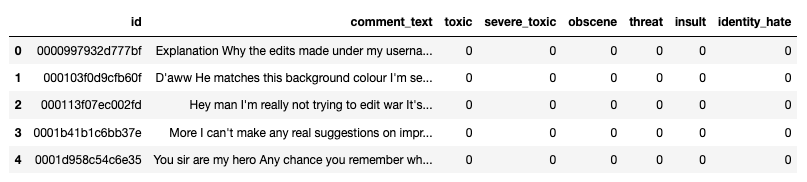
\includegraphics[width=140mm]{../local/plots_tables/train_head.png}
  \caption{Training dataset}
  \label{fig:train_head}
\end{figure}
The most occurrent words corresponding to the labels are in fact shown in the tittle page of this document.


\section{Exploratory Visualisation}


The data exploration is presented on \emph{/local/preprocessing\_exploration.ipynb}. 
The training set is distributed according to Fig.~\ref{fig:bar_plot}. It is extremly imbalanced. 
\begin{figure}[!h]
  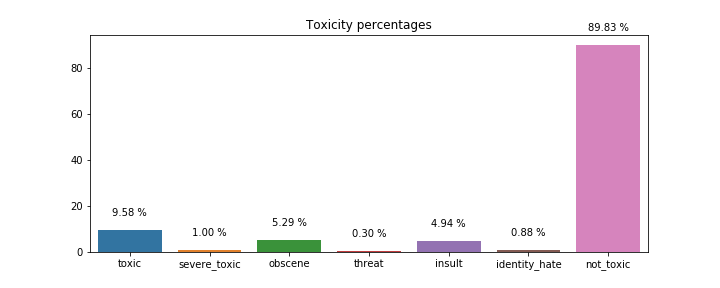
\includegraphics[width=\textwidth]{../local/plots_tables/bar_plot.png}
  \caption{Distribution of the different labels on training set}
  \label{fig:bar_plot}
\end{figure}
The correlations of the labels are shown in Fig.~\ref{fig:corr}
\begin{figure}[!h]
\centering
  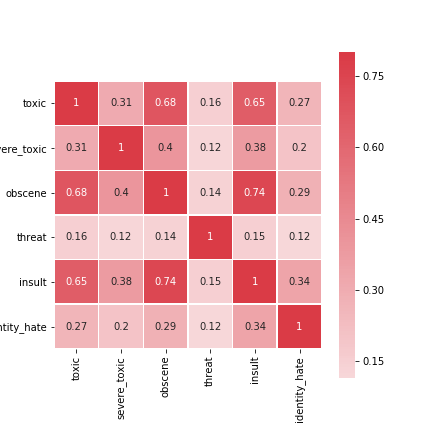
\includegraphics[width=80mm]{../local/plots_tables/corr.png}
  \caption{Correlations coefficients between labels}
  \label{fig:corr}
\end{figure}
Some correlations are large. But since we will predict each class independently this is not a problem. The histogram number of words distribution of the training set comments is presented on Fig.~\ref{fig:hist}. 
\begin{figure}[!h]
\centering
  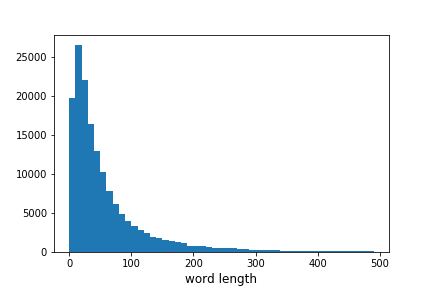
\includegraphics[width=100mm]{../local/plots_tables/word_length_hist.png}
  \caption{Number of words}
  \label{fig:hist}
\end{figure}
There are text which are clearly much longer but the vast majority is actually around 80 words as the cat plots in Fig.~\ref{fig:catplots}.
\begin{figure}[!h]
\centering
  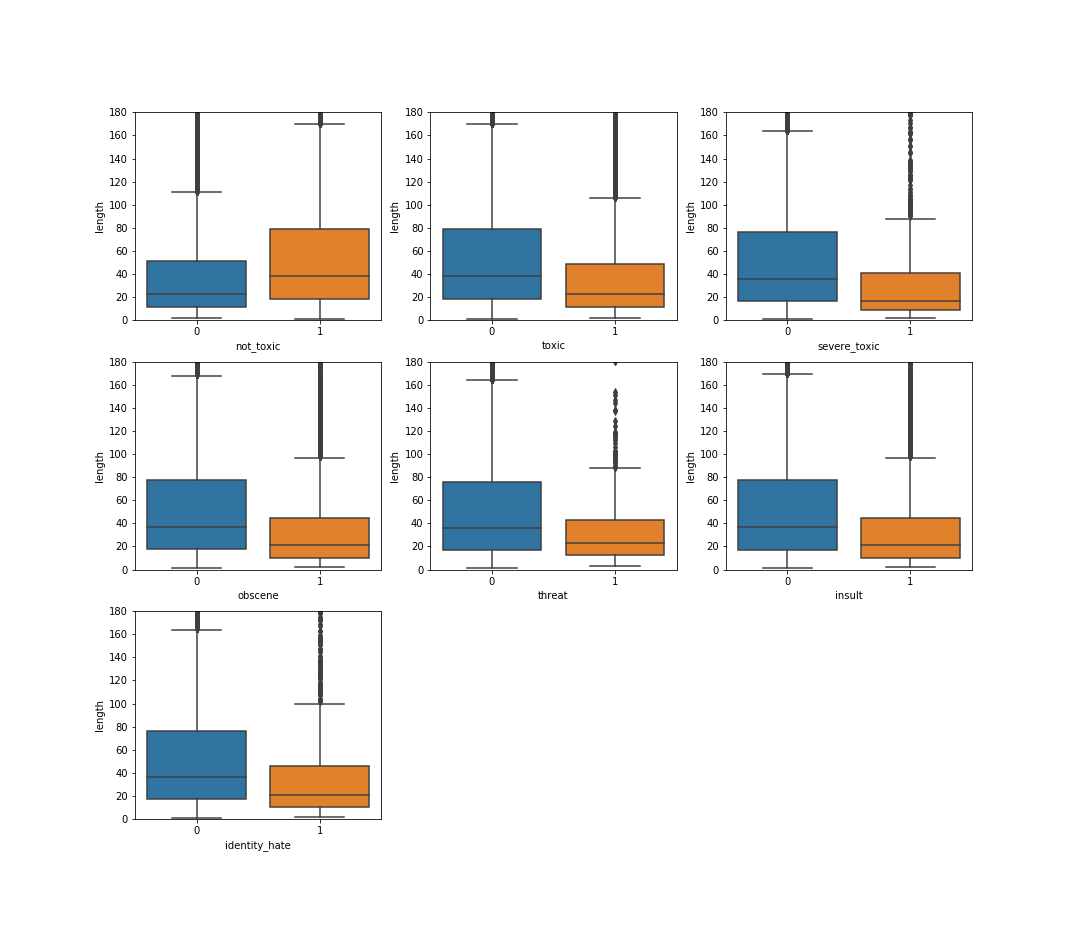
\includegraphics[width=170mm]{../local/plots_tables/catplots.png}
  \caption{Boxplots of number of words}
  \label{fig:catplots}
\end{figure}

\section{Algorithms and Techniques}

We studied three algorithmic techniques of deep learning architectures for natural
language processing. Before applying such architectures we applied the following 
text manipulations over the text:
\begin{enumerate}
\item Removed special characters except for numbers and apostrophes, which
were kept according to the english grammar rules.
\item Substitute any numerical character by letter n.
\item Reduce long comments to 80 words. This choice improved our metric 
and it was justified by observing the catplots of Fig.~\ref{fig:hist}. Indeed, 
most comments have 80 or less words. Interestingly most toxic comments tend 
to be shorten than 40 words long.
\end{enumerate}
The next steps were implemented using the \href{https://torchtext.readthedocs.io/en/latest/}{Torchtext package}. 
\begin{enumerate}
 \setcounter{enumi}{3}
\item Removing stopwords was attempted but in fact this slightly reduced the
accuracy obtained. 
\item Reducing words to their stemmed also slightly lower our evaluation metric.
\item Tokenization was implemented using the \href{https://scipy.org/scipylib/}{Spicy package}.


\item Comments were supplied in batches of 256 comments to all models. Dataset 
comments with similar number of words were grouped together, and padded, such that 
each batch had elements with identical number of words. It is worth remarking that this is
easily achieved by Torchtext and that we choose models compatible with this choice. Different 
batches sizes were attempted but 256 delivered the best evaluation metric performance. 

\item Finally, we embedded the training vocabulary into the glove.6B.100d embedding 
provided by torchtext, with a vocabulary of the 20000 most common words on the
training set, plust 

Finally, the following three model architectures were attempted:
\item Long-Short-Term-Memory, see \cite{NG} for an introduction to this model. We used the 
bidirectional version with two units. 


\end{enumerate}


\subsection{Benchmark}

As a bechmark for comparison we chose the most voted kernel of the respective 
Kaggle competition, which can be found in detail in this 
\href{https://www.kaggle.com/jhoward/nb-svm-strong-linear-baseline}{link}. In a nutshell, 
shows how to use Naive Bayes - Support Vector Machine (NBSVM) to create a strong baseline for this competition. 
A thorough description of this model can be found at \href{https://www.youtube.com/watch?v=37sFIak42Sc&feature=youtu.be&t=3745}{NBSVM}. It is worth noticing that the preprocessing is so
simple that stopwords are not removed and words are not stemmed. The main feature of this 
benchmark is its simplicity, we shall paired agains well tested strategies deep learning techniques.

\section{Datasets and inputs}

 

\section{Solution statement}

There are several competitive models developed in this competition. Rather than focusing 
on creating a model to reach the accuracy of top competitors, which may involve ensemble 
techniques as well as vast computational  resources, we shall focus on the task 
of creating developing models that can be train, deployed and updated on SageMaker,
emulating a production setting. To this end, 
I propose to use three well tested deep learning strategies on natural Language processing:

\begin{itemize}
\item Long short-term memory
\item Gated recurrent units
\item Convolutional neural networks
\end{itemize}
 
Of course, on the road we shall tackle text preprocessing and a choice of
pre-trained word embedding. We will use Pytorch as model build library as 
it is easy to train locally and it facilitates deployment on SageMaker.
 
\section{Benchmark model}

The metric of this multi-label Kaggle classification challenge 
uses the average of the  Area Under the Receiver Operating Characteristic Curve (ROC AUC) to 
 classify solutions. Currently, the team leading this competition scored team 0.98856\%.

As explained above, we aim to emulate a production 
environment not only for this particular problem but applied to other similar text
classification settings. Hence it is reasonable to demand our model reach the modest 97\% ROC AUC, 
but creating code that is easily trained, deployed and updated via Sagemaker. Furthermore, our 
models should be versatile enough that further improvements are easily achivable and 
generalisable to other classification settings, e g. modifying the network architecture and hyper-parameters 
must be easy.

\section{A set of evaluation metrics}

Our performance evaluation metric will be the class averaged, ROC AUC. Roughtly speaking, it measures 
how a model's probabilities separate the positive classes  from the negative classes and, crucially,
is a metric that asses a model regardless of the threshold chosen to map probabilities into categories. In addition, our aim 
is that the model is compact enough to perform on laptop cpu in around one hour (without hyperparameter tuning). 
Our non-quantitative metric is to create a metric that can be deployed with SageMaker, which can be easily improvable and updated by further work.


\section{An outline of the project design}

We shall use the contents of the Udacity nanodegree contents \cite{ND}, 
the course on Sequence Models by Andrew NG \cite{NG}, and the 
Ben Trevett tutorial  series on sentiment analysis \cite{BT} to follow the following program:
\begin{itemize}
\item Data Exploration (Pandas)
\item Text preprocessing (Spacy \cite{Spacy})
\item Choosing an appropriate word-embedding (Torchtext)
\item Try different well established models such as LSTM, GRU, Convolutional Networks (Pytorch)
\item Deployment via Sagemaker.
\end{itemize}

\bibliographystyle{unsrt}
\bibliography{qcd22}

\end{document}
